\documentclass[10pt]{article}

%defines page size and margins
\usepackage{geometry}
\geometry{
    letterpaper,
    left=1in,
    right=1in,
    top=1in,
    bottom=1in,
}

%Sets spacing for entire document
\usepackage{setspace}
\singlespacing

%Package for reducing space in between list items
\usepackage{enumitem}

%Math symbols
\usepackage{gensymb}
\usepackage{siunitx}

%Image path
\usepackage{graphicx}
\graphicspath{ {/} }

%Used for adjusting images
\usepackage[export]{adjustbox}

%For floating images
\usepackage{float}

\begin{document}
\title{Laboratory Four --- OP Amps}
\date{November 3, 2017}
\author{Rishabh Shah\\ 4655 4192\\ \\ Partner: Matthew Remillard}
\maketitle
\newpage

\section*{Pre-Lab}

\section*{Lab Data}
\subsection*{Voltage Follower}
\begin{table}[H]
	\centering
	\begin{tabular}{lll}
		\hline
		$V_{in}$ & $V_{CC}$ & $V_{out}$\\
		\hline
		$4.997V$ & $8.00V$ & $3.369V$\\
		\hline
	\end{tabular}
	\caption{Voltage follower data}
\end{table}

\subsection*{Inverting Amplifier}
$R_X = 58475 \Omega$
\begin{figure}[H]
	\centering
	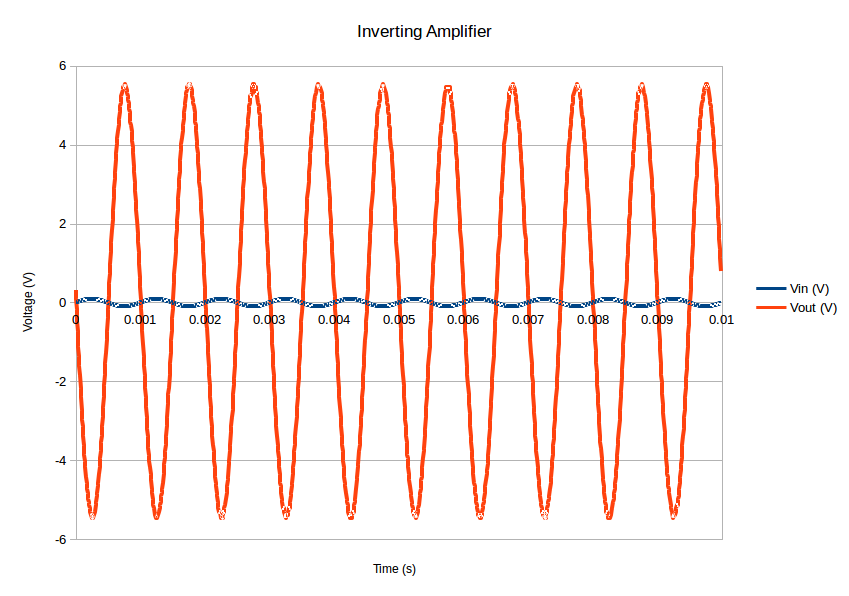
\includegraphics[width=\textwidth]{InvertingAmp.png}
	\caption{$V_{in}$ and $V_{out}$ vs Time for the inverting amplifier}
\end{figure}

\subsection*{Noninverting Amplifier}
$R_X = 105820 \Omega$
\begin{figure}[H]
	\centering
	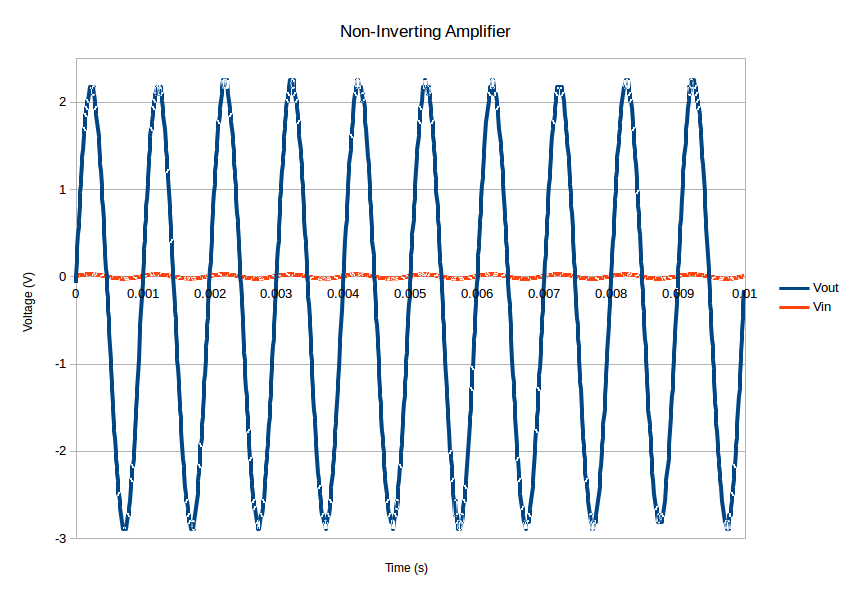
\includegraphics[width=\textwidth]{NonInvertingAmp.png}
	\caption{$V_{in}$ and $V_{out}$ vs Time for the noninverting amplifier}
\end{figure}

\subsection*{Clipping}
\begin{table}[H]
	\centering
	\begin{tabular}{llllll}
		\hline
		$+V_{CC}(V)$ & $-V_{CC}(V)$ & $V_{OUT,MAX}(V)$ & $V_{OUT,MIN}(V)$ & $\Delta V+(V)$ & $\Delta V-(V)$\\
		\hline
		15 & -15 & 13.1 & -13.3 & 1.9 & -1.7\\
		20 & -20 & 17.7 & -17.9 & 2.3 & -2.1\\
		\hline
	\end{tabular}
	\caption{Data when $R_L=2k\Omega$}
\end{table}
\begin{figure}[H]
	\centering
	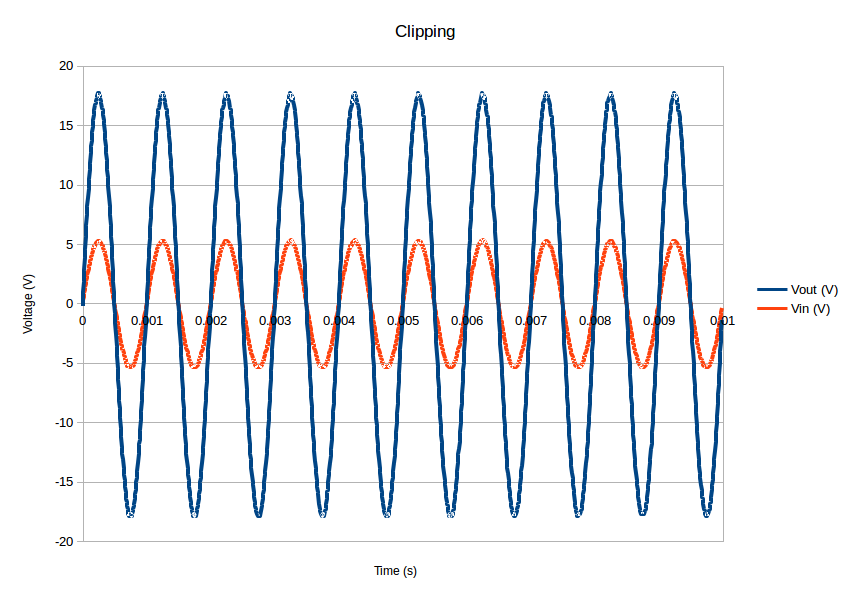
\includegraphics[width=\textwidth]{Clipping20V1.png}
	\caption{$V_{in}$ and $V_{out}$ vs Time for when $R_L=2k\Omega$}
\end{figure}
\begin{table}[H]
	\centering
	\begin{tabular}{llllll}
		\hline
		$+V_{CC}(V)$ & $-V_{CC}(V)$ & $V_{OUT,MAX}(V)$ & $V_{OUT,MIN}(V)$ & $\Delta V+(V)$ & $\Delta V-(V)$\\
		\hline
		15 & -15 & 13.3 & -13.7 & 1.7 & -1.3\\
		20 & -20 & 18.1 & -18.3 & 1.9 & -1.7\\
		\hline
	\end{tabular}
	\caption{Data when $R_L=10k\Omega$}
\end{table}
\begin{figure}[H]
	\centering
	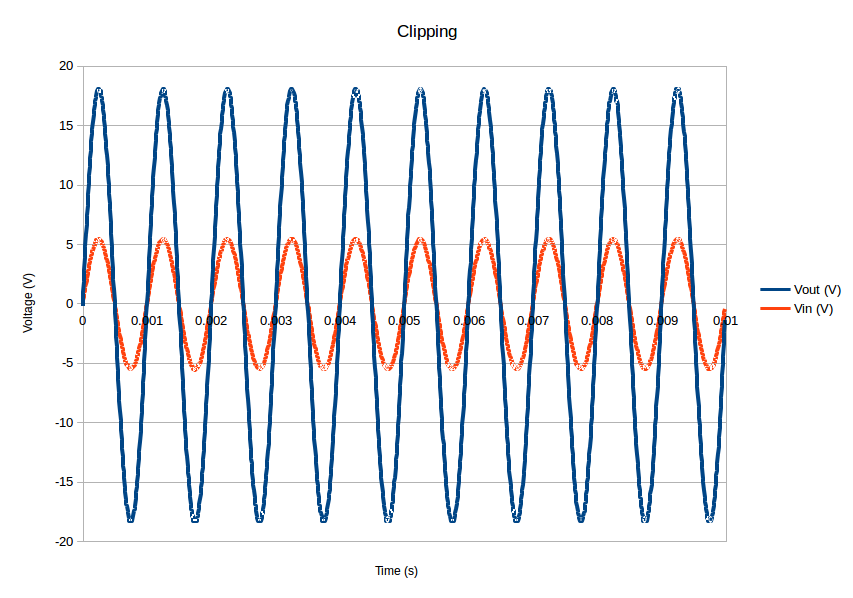
\includegraphics[width=\textwidth]{Clipping20V2.png}
	\caption{$V_{in}$ and $V_{out}$ vs Time for when $R_L=10k\Omega$}
\end{figure}

\subsection*{Phase Shift and Time Delay}
\begin{table}[H]
	\centering
	\begin{tabular}{lll}
		\hline
		Frequency $(kHz)$ & Shift $(\mu s)$ & Shift $(\degree)$\\
		\hline
		2 & -13.3 & -5.38\\
		5 & -11.6 & -20.5\\
		10 & -9.6 & -36.3\\
		20 & -7.9 & -57.2\\
		\hline
	\end{tabular}
	\caption{Data for phase shift and time delay}
\end{table}
\begin{figure}[H]
	\centering
	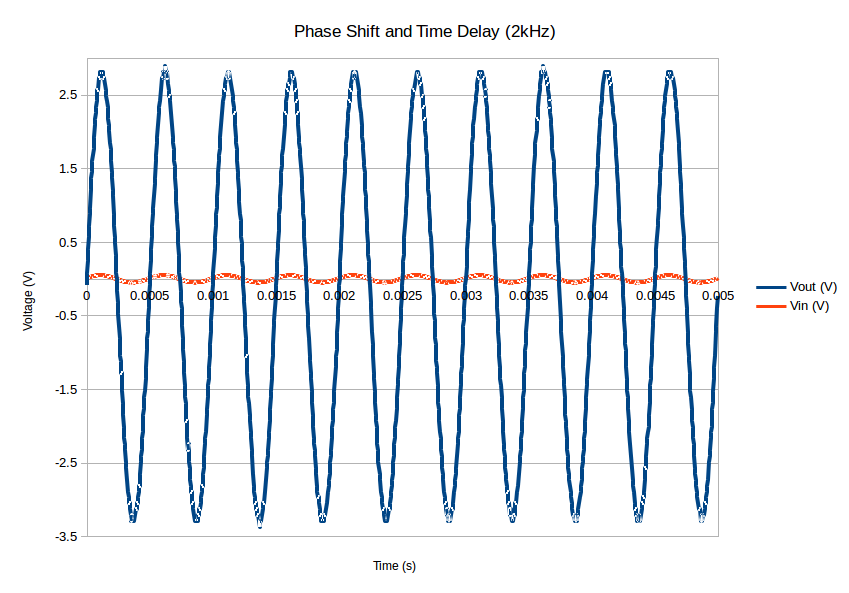
\includegraphics[width=\textwidth]{PhaseShift2.png}
	\caption{$V_{in}$ and $V_{out}$ vs Time for when frequency is $2kHz$}
\end{figure}
\begin{figure}[H]
	\centering
	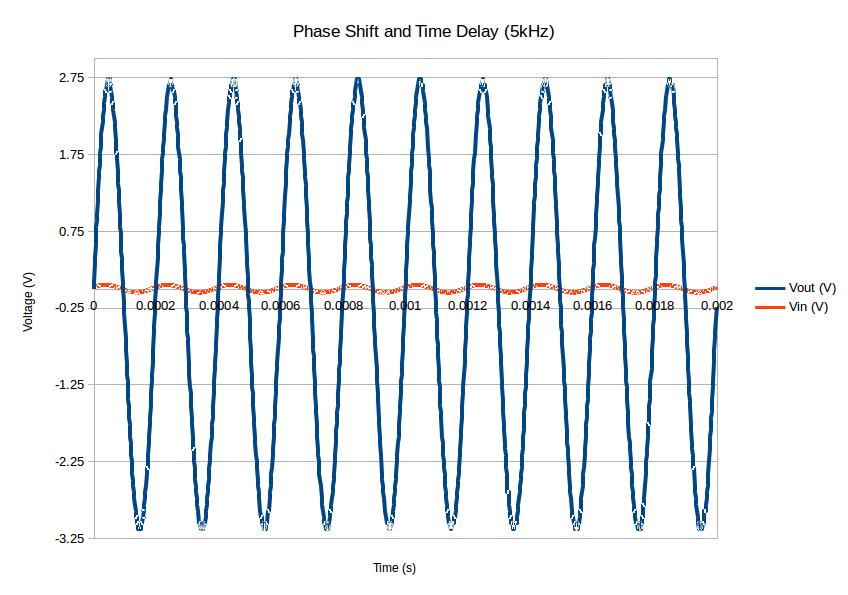
\includegraphics[width=\textwidth]{PhaseShift5.png}
	\caption{$V_{in}$ and $V_{out}$ vs Time for when frequency is $5kHz$}
\end{figure}
\begin{figure}[H]
	\centering
	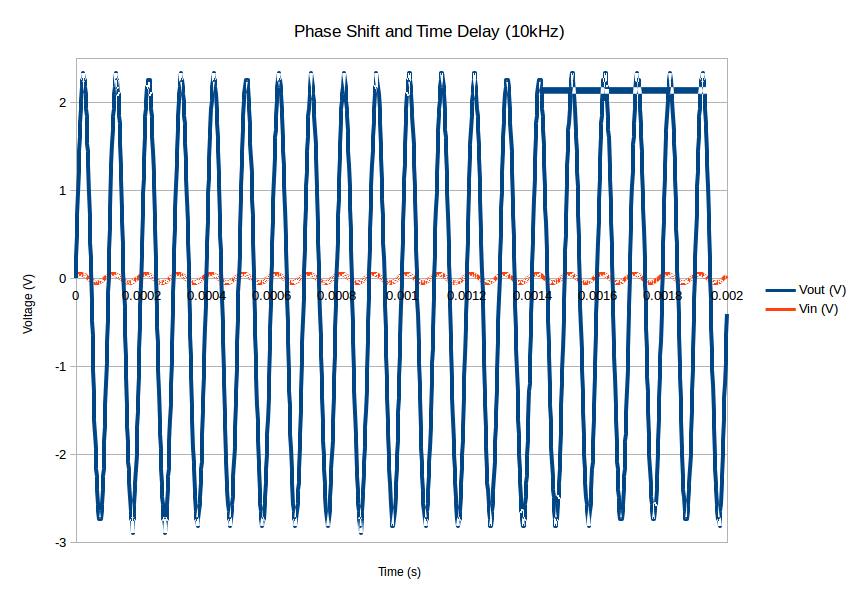
\includegraphics[width=\textwidth]{PhaseShift10.png}
	\caption{$V_{in}$ and $V_{out}$ vs Time for when frequency is $10kHz$}
\end{figure}
\begin{figure}[H]
	\centering
	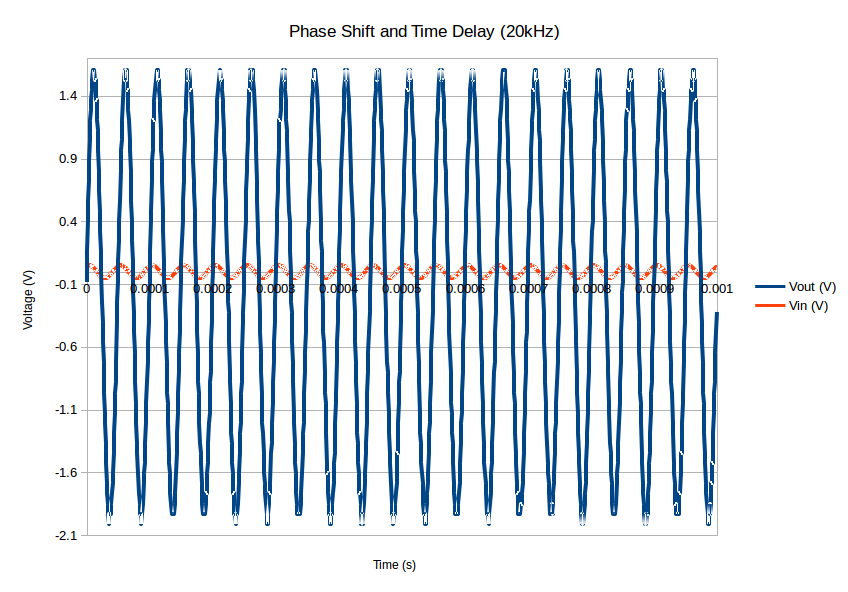
\includegraphics[width=\textwidth]{PhaseShift20.png}
	\caption{$V_{in}$ and $V_{out}$ vs Time for when frequency is $20kHz$}
\end{figure}

\section*{Post-Lab}
\subsection*{Voltage Buffer}
\noindent Using ideal op-amp assumptions, $V_{out} = V_{in}$ in a voltage follower circuit due to 100\% negative feedback.
$$V_{in} = \frac{V_S}{R_1 + R_2} R_2 = \frac{5V}{100k\Omega + 200k\Omega}200k\Omega = 3.333V$$
$$Percentage Error = \frac{|measured-calculated|}{calculated} = \frac{|3.369V-3.333V|}{3.333V} = 1.080\%$$
\noindent If the value of $R_3$ changed, it would have an effect on the current drawn from the voltage source. If the value of $R_3$ increases, the current drawn would decrease. If the value of $R_3$ decreases, the current drawn would increase.

\subsection*{Inverting Amplifier}
\noindent Using ideal op-amp assumptions,
$$Gain = \frac{V_{out}}{V_{in}}$$
$$V_{out} = \frac{R_f}{R_{S}}V_{in}$$
$$R_f = |Gain| \cdot R_{S} = 50 \cdot 1000\Omega = 50k\Omega$$
$$Percentage Error = \frac{|measured-calculated|}{calculated} = \frac{|59475\Omega-50000\Omega|}{50000\Omega} = 18.95\%$$
\noindent The measured $R_f$ was larger than the calculated value by $18.95\%$. This is due to the fact that the calculated value relied on an ideal op-amp. However, the op-amp used in the experiment was not an ideal op-amp. The LM 741 is a non-ideal op-amp, causing the difference between the calculated and measured values.

\subsection*{Noninverting Amplifier}
\noindent Using ideal op-amp assumptions,
$$Gain = \frac{V_{out}}{V_{in}}$$
$$V_{out} = (1+\frac{R_f}{R_{S}})V_{in}$$
$$R_f = (|Gain|-1)\cdot R_{S} = (100-1)\cdot 1k\Omega = 99k\Omega$$
$$Percentage Error = \frac{|measured-calculated|}{calculated} = \frac{|106820\Omega-99000\Omega|}{99000\Omega} = 7.90\%$$
\noindent The measured $R_f$ was larger than the calculated value by $7.90\%$. This is due to the fact that the calculated value relied on an ideal op-amp. However, the op-amp used in the experiment was not an ideal op-amp. The LM 741 is a non-ideal op-amp, causing the difference between the calculated and measured values.

\subsection*{Clipping}

\subsection*{Phase Shift}
\noindent As the frequency increased, the phase shift in $\mu s$ increased but the magnitude of the phase shift in $\mu s$ decreased. The phase shift in degrees decreased but the magnitude of the phase shift in degrees increased. 
\end{document}